\documentclass[11pt]{article}
\usepackage[utf8]{inputenc}
\usepackage[T1]{fontenc}
\usepackage{amsmath}
\usepackage{multicol}
\usepackage{geometry}
\usepackage{tikz}
\usetikzlibrary{shapes.geometric, arrows.meta, calc, patterns}
\usepackage{enumitem}
\usepackage{xcolor}
\usepackage{titlesec}

% Configurações de layout
\geometry{a4paper, left=1cm, right=1cm, top=0.5cm, bottom=1.2cm}
\setlength{\columnseprule}{0.4pt}
\setlength{\baselineskip}{1.0\baselineskip}

% Cores personalizadas
\definecolor{titleblue}{RGB}{0,80,150}
\definecolor{sectionred}{RGB}{180,0,0}
\definecolor{darkgreen}{RGB}{0,100,0}
\definecolor{examplecolor}{RGB}{50,100,150}

% Formatação de títulos
\titleformat{\section}{\normalfont\Large\bfseries\color{titleblue}}{\thesection}{1em}{}
\titleformat{\subsection}{\normalfont\large\bfseries\color{sectionred}}{\thesubsection}{1em}{}
\titleformat{\subsubsection}{\normalfont\normalsize\bfseries\color{darkgreen}}{\thesubsubsection}{1em}{}

\title{\textcolor{titleblue}{Geometria: Perímetro de Figuras Planas}}
\author{Professor: Jefferson}
\date{}

\begin{document}

\maketitle
\vspace{-1cm}

\begin{center}
\large{Nome: \underline{\hspace{8cm}} \quad Turma: \underline{\hspace{3cm}}}
\end{center}

\begin{multicols}{2}

\section*{1. Conceito de Perímetro}
O perímetro é a medida do \textbf{contorno} de uma figura plana, ou seja, a soma dos comprimentos de todos os seus lados.

\begin{center}
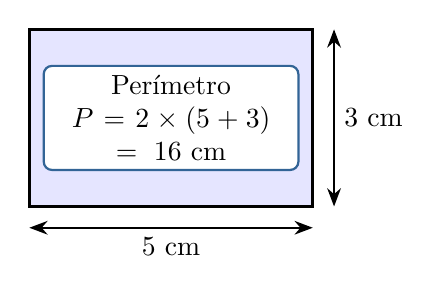
\begin{tikzpicture}[scale=0.9]
    \draw[very thick, fill=blue!10] (0,0) -- (4,0) -- (4,2.5) -- (0,2.5) -- cycle;
    \draw[<->, >=Stealth, line width=0.8pt] (0,-0.3) -- (4,-0.3) node[midway,below] {5 cm};
    \draw[<->, >=Stealth, line width=0.8pt] (4.3,0) -- (4.3,2.5) node[midway,right] {3 cm};
    \node[align=center, text width=3cm, fill=white, rounded corners=3pt, draw=examplecolor, thick] at (2,1.25) {Perímetro \\ $P = 2\times(5+3)$ \\ $= 16$ cm};
\end{tikzpicture}
\end{center}

\section*{2. Perímetro de Figuras Básicas}

\subsection*{2.1 Quadrado}
\begin{itemize}
    \item Todos os lados iguais
    \item Fórmula: $P = 4 \times L$
\end{itemize}

\begin{center}
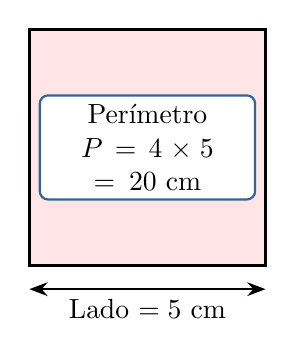
\begin{tikzpicture}[scale=1.0]
    \draw[very thick, fill=red!10] (0,0) -- (3,0) -- (3,3) -- (0,3) -- cycle;
    \draw[<->, >=Stealth, line width=0.8pt] (0,-0.3) -- (3,-0.3) node[midway,below] {Lado $= 5$ cm};
    \node[align=center, text width=2.5cm, fill=white, rounded corners=3pt, draw=examplecolor, thick] at (1.5,1.5) {Perímetro \\ $P = 4 \times 5$ \\ $= 20$ cm};
\end{tikzpicture}
\end{center}

\subsection*{2.2 Retângulo}
\begin{itemize}
    \item Lados opostos iguais
    \item Fórmula: $P = 2 \times (b + h)$
\end{itemize}

\begin{center}
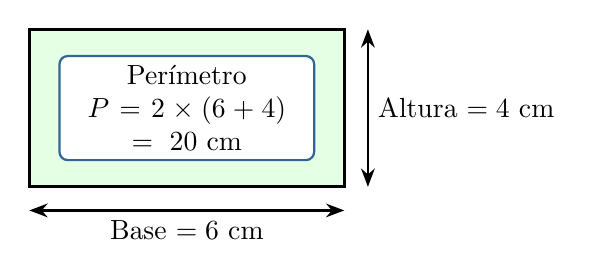
\begin{tikzpicture}[scale=1.0]
    \draw[very thick, fill=green!10] (0,0) -- (4,0) -- (4,2) -- (0,2) -- cycle;
    \draw[<->, >=Stealth, line width=0.8pt] (0,-0.3) -- (4,-0.3) node[midway,below] {Base $= 6$ cm};
    \draw[<->, >=Stealth, line width=0.8pt] (4.3,0) -- (4.3,2) node[midway,right] {Altura $= 4$ cm};
    \node[align=center, text width=3cm, fill=white, rounded corners=3pt, draw=examplecolor, thick] at (2,1) {Perímetro \\ $P = 2\times(6+4)$ \\ $= 20$ cm};
\end{tikzpicture}
\end{center}

\subsection*{2.3 Triângulo}
\begin{itemize}
    \item Soma dos três lados
    \item Fórmula: $P = a + b + c$
\end{itemize}

\begin{center}
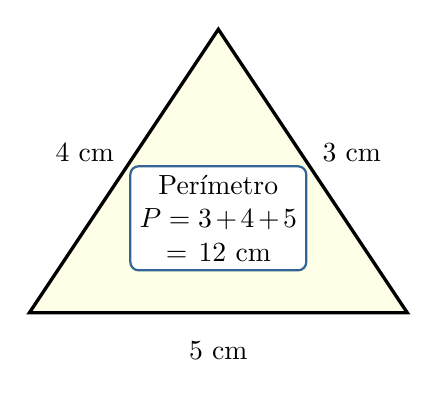
\begin{tikzpicture}[scale=1.2]
    \draw[very thick, fill=yellow!10] (0,0) -- (4,0) -- (2,3) -- cycle;
    \node[below] at (2,-0.2) {5 cm};
    \node[above left] at (1,1.5) {4 cm};
    \node[above right] at (3,1.5) {3 cm};
    \node[align=center, text width=2cm, fill=white, rounded corners=3pt, draw=examplecolor, thick] at (2,1) {Perímetro \\ $P = 3+4+5$ \\ $= 12$ cm};
\end{tikzpicture}
\end{center}

\subsection*{2.4 Círculo (Circunferência)}
\begin{itemize}
    \item Chamado de circunferência
    \item Fórmula: $C = 2\pi r = \pi d$
\end{itemize}

\begin{center}
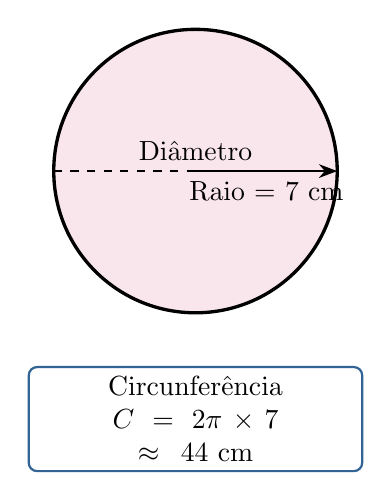
\begin{tikzpicture}[scale=0.9]
    \draw[very thick, fill=purple!10] (0,0) circle (2);
    \draw[->, >=Stealth, line width=0.8pt] (0,0) -- (2,0) node[midway,below] {Raio = 7 cm};
    \draw[dashed, thick] (-2,0) -- (2,0) node[midway,above] {Diâmetro};
    \node[align=center, text width=4cm, fill=white, rounded corners=3pt, draw=examplecolor, thick] at (0,-3.5) {Circunferência \\ $C = 2\pi \times 7$ \\ $\approx 44$ cm};
\end{tikzpicture}
\end{center}

\section*{3. Perímetro de Polígonos Regulares}
Polígonos regulares têm todos os lados e ângulos iguais.

\subsection*{Fórmula Geral}
$P = n \times L$ \\
onde $n$ = número de lados, $L$ = comprimento de cada lado

\begin{center}
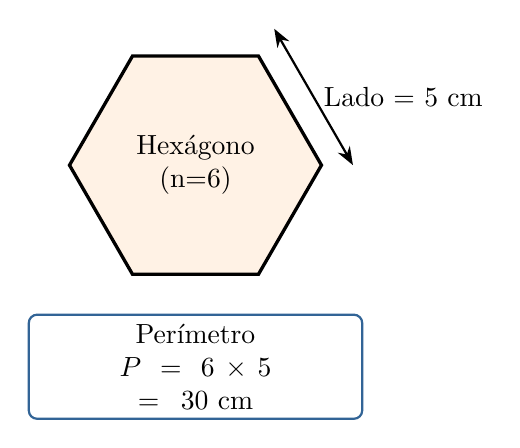
\begin{tikzpicture}[scale=0.8]
    \draw[very thick, fill=orange!10] (0:2) -- (60:2) -- (120:2) -- (180:2) -- (240:2) -- (300:2) -- cycle;
    \node[align=center] at (0,0) {Hexágono \\ (n=6)};
    \draw[<->, >=Stealth, line width=0.8pt] (0:2.5) -- (60:2.5) node[midway,right] {Lado = 5 cm};
    \node[align=center, text width=4cm, fill=white, rounded corners=3pt, draw=examplecolor, thick] at (0,-3.2) {Perímetro \\ $P = 6 \times 5$ \\ $= 30$ cm};
\end{tikzpicture}
\end{center}

\section*{4. Aplicações Práticas}

\subsection*{4.1 Cercando Terrenos}
Calcular o comprimento de cerca necessário para um terreno retangular de 25m × 40m.

\begin{center}
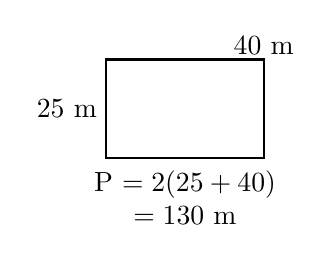
\begin{tikzpicture}[scale=0.5]
    \draw[thick] (0,0) rectangle (4,2.5);
    \node at (-1,1.25) {25 m};
    \node at (4.0,2.85) {40 m};
    \node[align=center] at (2,-1) {P $= 2×(25+40)$ \\ $= 130$ m};
\end{tikzpicture}
\end{center}

\subsection*{4.2 Molduras para Quadros}
Determinar o comprimento de moldura para um quadro quadrado de 30 cm de lado.

\begin{center}
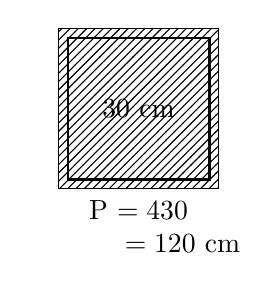
\begin{tikzpicture}[scale=0.6]
    \draw[thick] (0,0) rectangle (3,3);
    \draw[pattern=north east lines] (-0.2,-0.2) rectangle (3.2,3.2);
    \node at (1.5,1.5) {30 cm};
    \node[align=center] at (1.5,-1) {P $= 4×30$ \\ \hspace{1cm} $= 120$ cm};
\end{tikzpicture}
\end{center}

\section*{5. Exercícios Básicos}

\begin{enumerate}
    \item Calcule o perímetro de:
    \begin{enumerate}[label=\alph*)]
        \item Um quadrado com lado de 8 cm
        \item Um retângulo com lados 5 m e 12 m
        \item Um triângulo equilátero com lado 6 cm
    \end{enumerate}
    
    \item Determine o perímetro de:
    \begin{enumerate}[label=\alph*)]
        \item Um pentágono regular com lado 4 cm
        \item Um círculo com raio 10 cm (use $\pi = 3,14$)
    \end{enumerate}
    
    \item Resolva:
    \begin{enumerate}[label=\alph*)]
        \item Se o perímetro de um quadrado é 36 cm, qual é seu lado?
        \item Um retângulo tem perímetro 30 m e altura 5 m. Qual sua base?
    \end{enumerate}
    
    \item Problemas:
    \begin{enumerate}[label=\alph*)]
        \item Quantos metros de cerca são necessários para um terreno triangular com lados 15 m, 20 m e 25 m?
        \item Uma pista circular tem 50 m de raio. Qual o comprimento de uma volta completa?
    \end{enumerate}
\end{enumerate}

\section*{6. Exercícios Intermediários}

\begin{enumerate}\setcounter{enumi}{4}
    \item Determine o lado que falta:
    \begin{enumerate}[label=\alph*)]
        \item Triângulo com $P=45$ cm e lados 15 cm e 20 cm
        \item Pentágono regular com $P=65$ cm
    \end{enumerate}
    
    \item Problemas aplicados:
    \begin{enumerate}[label=\alph*)]
        \item Uma praça circular tem circunferência de 188,4 m. Qual seu raio?
        \item Para cercar um terreno retangular gastou-se 120 m de arame. Se a largura é 20 m, qual o comprimento?
    \end{enumerate}
    
    \item Desafios:
    \begin{enumerate}[label=\alph*)]
        \item Um quadrado e um triângulo equilátero têm o mesmo perímetro. Se o lado do quadrado é 6 cm, qual o lado do triângulo?
        \item Quantas voltas dá uma roda de 35 cm de raio para percorrer 220 m?
    \end{enumerate}
\end{enumerate}

\section*{7. Tabela Resumo}

\begin{center}
\begin{tabular}{|l|c|c|}
\hline
\textbf{Figura} & \textbf{Fórmula} & \textbf{Exemplo} \\
\hline
Quadrado & $P = 4L$ & $L=5$ → $P=20$ \\
Retângulo & $P = 2(b+h)$ & $b=6$,$h=4$ → P=20 \\
Triângulo & $P = a+b+c$ & 3,4,5 → $P=12$ \\
Círculo & $C = 2\pi r$ & $r=7$ → $C≈44$ \\
n-ágono regular & $P = nL$ & $n=5$,$L=4$ → $P=20$ \\
\hline
\end{tabular}
\end{center}


\end{multicols}

\end{document}
